\documentclass{beamer}

\usepackage{amsmath, amssymb}
\usepackage{tikz-cd}
\usepackage{xcolor}
\usepackage{graphicx}

\title{MT222: Calculus II}
\author{\textbf{Miraj Samarakkody}}
\institute{Tougaloo College}
\date{03/28/2025}

\begin{document}

\begin{frame}
    \titlepage
\end{frame}




\begin{frame}{}
    \begin{center}
        \Huge{7.3 - Trigonometric Substitution}
    \end{center}
    
\end{frame}



\begin{frame}{Table of Trigonometric Substitiution}
    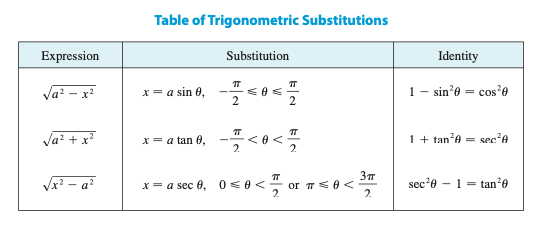
\includegraphics[scale=0.6]{figures/fig_1.png}
\end{frame}


\begin{frame}{Example 3}
    Find \[\int \dfrac{1}{x^2 \sqrt{x^2+4}}~dx\]
\end{frame}

\begin{frame}{Example 4}
    Find \[\int \dfrac{x}{\sqrt{x^2+4}}dx\]
\end{frame}

\begin{frame}{Example 5}
    Evaluate \[\int \dfrac{dx}{\sqrt{x^2-a^2}},\] where \(a>0\).
    
\end{frame}

\begin{frame}{Example 5}
    Evaluate \[\int \dfrac{dx}{\sqrt{x^2-a^2}},\] where \(a>0\). (Use Hyperbolic functions)
    
\end{frame}

\begin{frame}{Example 6}
    Find \[\int_{0}^{3\sqrt{3}/2}\dfrac{x^3}{(4x^2+9)^{3/2}}dx\]
\end{frame}

\begin{frame}{Example 7}
    Evaluate \[\int \dfrac{x}{\sqrt{3-2x-x^2}}dx\]
\end{frame}

\begin{frame}{}
\begin{center}
    \Huge{Integration of Rational Functions by Partial Fractions}
\end{center}
\end{frame}

\begin{frame}{Motivation}
In this section, we show how to integrate any rational function by expressing it as a sum of simpler fractions, called \textit{partial fraction}, that we already know how to integrate. 
\end{frame}

    \begin{frame}{Example 1}
    Find \[\int \dfrac{x^3+x}{x-1}~dx\]\\ \pause
    \vspace{0.5in}
    Next we study some different cases. 
    \end{frame}

\begin{frame}{CASE I: The denominator \(Q(x)\) is a product of distinct linear factors.}    
We can write \[Q(x)=(a_1 x+b_1)(a_2x+b_2)\dots (a_k x +b_k),\] where no factor is repeated. \\ \pause
\vspace{0.2in}
In this case the partial fraction theorem states that there exist constants \(A_1,A_2,A_3, \dots , A_k\) such that \[\dfrac{R(x)}{Q(x)}= \dfrac{A_1}{a_1x+b_1}+ \dfrac{A_2}{a_2x+b_2}+ \dots + \dfrac{A_k}{a_k x +b_k}.\]
\end{frame}

\begin{frame}{Example 2}
Write the partial fraction decomposition of \[\dfrac{x^2 +2x -1}{2x^3+3x^2-2x}\]
\end{frame}

\begin{frame}{Example 2}
    Use and alternative method to write the partial fraction decomposition of \[\dfrac{x^2 +2x -1}{2x^3+3x^2-2x}\]
    \end{frame}

\begin{frame}{Example 2}
Find \[\int \dfrac{x^2 +2x -1}{2x^3+3x^2-2x}dx\]
\end{frame}

\begin{frame}{Example 3}
Find \[\int \dfrac{x^2-a^2}{dx},\] where \(a \ne 0\).
\end{frame}

\begin{frame}{CASE II: \(Q(x)\) is a product of linear factors, some of which are repeated.}
Suppose the first linear factor \((a_1 x+b_1)\) is repeated \(r\) times; that is, \((a_1 x +b_1)^r\) occurs in the factorization of \(Q(x)\). Then instead of the single term \(\dfrac{A_1}{(a_1 x+b)}\), we would write 
\[\dfrac{A_1}{(a_1 x+b)}+\dfrac{A_2}{(a_1 x+b)^2}+\dots + \dfrac{A_r}{(a_1 x+b)^r}\]
\end{frame}

\begin{frame}{Example 4}
Find \[\int \dfrac{x^4 -2x^2 +4x +1}{x^3 -x^2 -x+1}~dx.\]
\end{frame}

\begin{frame}{Case III: \(Q(x)\) contains irreducible quadratic factors, none of which is repeated. }
If \(Q(x)\) has the factor \(ax^2 +bx +c\), where \(b^2 -4ac <0\), then the expression for \(R(x)/Q(x)\) will have a term of the form \[\dfrac{Ax+B}{ax^2 +bx +c},\] 
\end{frame}

\begin{frame}{Example 5}
Evaluate \[\int \dfrac{2x^2 -x +4}{x^3+4x}~dx\]
\end{frame}

\begin{frame}{Example 6}
Evaluate \[\int \dfrac{4x^2 -3x +2}{4x^2-4x+3}~dx\]
\end{frame}

\begin{frame}{Case IV: \(Q(x)\) contains a repeated irreducible quadratic factor.}
If \(Q(x)\) has the factor \((ax^2+bx+c)^r\), where \(b^2 -4ac<0\), then instead of the single partial fraction, the sum \[\dfrac{A_1x +B_1}{ax^2+bx+c}+\dfrac{A_2x +B_2}{(ax^2+bx+c)^2}+\dots+\dfrac{A_rx +B_r}{(ax^2+bx+c)^r}\]

occurs in the partial fraction decomposition of \(R(x)/Q(x)\).
\end{frame}

\begin{frame}{Example 7}
Write out the form of the partial fraction decomposition of the function \[
\dfrac{x^3 +x^2 +1}{x(x-1)(x^2+x+1)(x^2+1)^3}
\]
\end{frame}

\begin{frame}{Example 8}
Evaluate \[
\int \dfrac{1-x+2x^2-x^3}{x(x^2+1)^2}dx
\]
\end{frame}

\begin{frame}{Rationalizing Substitutions}
Some non-rational functions can be changed into rational functions by means of appropriate substitutions. 
\begin{block}{Example 9}
Evaluate \[\int \dfrac{\sqrt{x+4}}{x}~dx.\]
\end{block}
\end{frame}




\end{document}